\chapter{Background and Literature Review}
\label{chap:background}

As organizations increasingly integrate artificial intelligence into their operational workflows, they face challenges in processing unstructured data streams effectively. In domains centered on human interaction, this includes chat logs, customer feedback, and support inquiries. This chapter presents the foundational concepts and methodologies relevant to building AI-driven systems capable of understanding and responding to human emotion, focusing on the theoretical foundations necessary for developing emotionally intelligent LLMs.

\noindent The chapter is structured to provide comprehensive coverage of the technical domains required for creating emotionally aware AI. The background section establishes theoretical foundations across key areas: psychological models of EI, the evolution of natural language processing techniques for affective computing, core algorithms for semantic analysis, and robust evaluation frameworks. The literature review then systematically analyzes existing research through a structured methodology to identify critical gaps and establish the motivation for the development of a novel hybrid solution.

\section{Background}

\subsection{Psychological and Computational Foundations of EI:} 
The pursuit of computational EI is fundamentally an effort to model and replicate aspects of human emotional processing. This requires grounding technical approaches in established psychological theories that define the construct of emotional intelligence itself.

\subsection{The Mayer-Salovey Model of Emotional Intelligence:} 
%% ENHANCEMENT: Added a stronger introductory sentence to frame the model's importance.
The most influential psychological framework for this purpose is the Mayer-Salovey model, which defines EI as a set of discrete cognitive abilities rather than merely personality traits \cite{salovey1990emotional, mayer1997what}. This ability-based model is particularly well-suited for guiding AI development, as it breaks EI down into four hierarchical branches of measurable skills:
\begin{enumerate}
    \item \textbf{Perceiving Emotions:} The foundational ability to accurately recognize emotions in oneself and others. For an LLM, this translates to the task of identifying affective cues in text, from explicit emotion words to nuanced sentiment expressed through syntax and semantics.
    \item \textbf{Using Emotions to Facilitate Thought:} The ability to leverage emotions to guide cognitive processes, such as problem-solving and creativity. An emotionally intelligent AI might use a detected user emotion (e.g., frustration) to adapt its response strategy, perhaps by simplifying its explanation or offering direct assistance.
    \item \textbf{Understanding Emotions:} The capacity to comprehend complex emotional language, the causes and consequences of emotions, and how emotions transition over time. This branch directly informs advanced NLP tasks like emotion cause extraction \cite{huang2023emotioncause} and empathetic reasoning.
    \item \textbf{Managing Emotions:} The highest-level ability, involving the regulation of one's own and others' emotions to achieve desired outcomes. In AI, this is most clearly manifested in empathetic dialogue systems designed to provide comfort, de-escalate conflict, or offer emotional support \cite{rashkin2019empathetic}.
\end{enumerate}
This model provides a clear, structured blueprint for what a truly emotionally intelligent AI should be capable of, moving beyond simple sentiment analysis to encompass a full spectrum of emotional reasoning and interaction.

\subsection{NLP Techniques for Emotion Recognition:} 
%% ENHANCEMENT: Added a citation to frame the evolution of NLP.
Natural Language Processing provides the technical toolkit to operationalize these psychological concepts. The field has seen remarkable advances, evolving from rule-based systems to sophisticated neural models capable of understanding context and nuance \cite{hirschberg2015advances}.

\subsubsection{Sentiment Analysis:}  This remains a foundational task, focused on classifying text into broad polarity categories (positive, negative, neutral). Modern LLMs have demonstrated exceptional performance in this area, often achieving high accuracy in zero-shot settings without task-specific training \cite{amin2023affective}.

\subsubsection{Fine-Grained Emotion Classification:}  This extends sentiment analysis by identifying a wider range of specific emotions (e.g., joy, anger, surprise). This task typically involves multi-label classification, as text can express a complex blend of feelings. The creation of large-scale annotated corpora like GoEmotions has been instrumental in benchmarking progress in this area \cite{demszky2020goemotions}.

\subsubsection{Emotion Cause Extraction (ECE):}  A more complex reasoning task, ECE aims to identify the specific events or statements that trigger an emotional response in text. This requires a model to understand not just affect, but causality. Recent approaches have focused on decomposing this problem into a chain of reasoning steps that are more tractable for LLMs \cite{wu2024decc}.

\subsubsection{Empathetic Dialogue Generation:}  Representing the pinnacle of applied computational EI, this task involves generating responses that are not only contextually relevant but also emotionally supportive and validating. Progress in this area relies on specialized datasets and models designed to learn the principles of empathetic communication, often incorporating explicit strategies for providing support \cite{liu2021esconv}.

\subsubsection{Data Structures and Granularity in Emotion Datasets:} 
%% ENHANCEMENT: Re-integrated the section on data structures from our previous discussion, as it is critical for your project's justification.
The effectiveness of any emotion recognition system is heavily dependent on the structure and quality of its underlying training data. Foundational datasets in affective computing are often designed with a hierarchical structure that reflects the psychological relationships between different emotions.

A prime example is the \textbf{GoEmotions dataset}, which has become a standard benchmark for fine-grained emotion classification \cite{demszky2020goemotions}. It contains 27 distinct emotion categories that are not mutually exclusive. As demonstrated by this study, these emotions can be organized through hierarchical clustering based on their co-occurrence and semantic similarity. This reveals a natural structure of positive, negative, and ambiguous emotion groups, as illustrated in Figure \ref{fig:goemotions_cluster}.

This hierarchical structure is not merely a descriptive feature; it provides a methodological basis for evaluating model performance at different levels of emotional granularity. An LLM can be tested on its ability to distinguish all 27 fine-grained emotions, its ability to classify text into broader emotional clusters, or its ability to perform high-level sentiment classification (positive, negative, ambiguous). This multi-granularity approach, which is a core component of this Capstone project, allows for a more comprehensive assessment of an LLM's emotional understanding.

\begin{figure}[H]
    \centering
    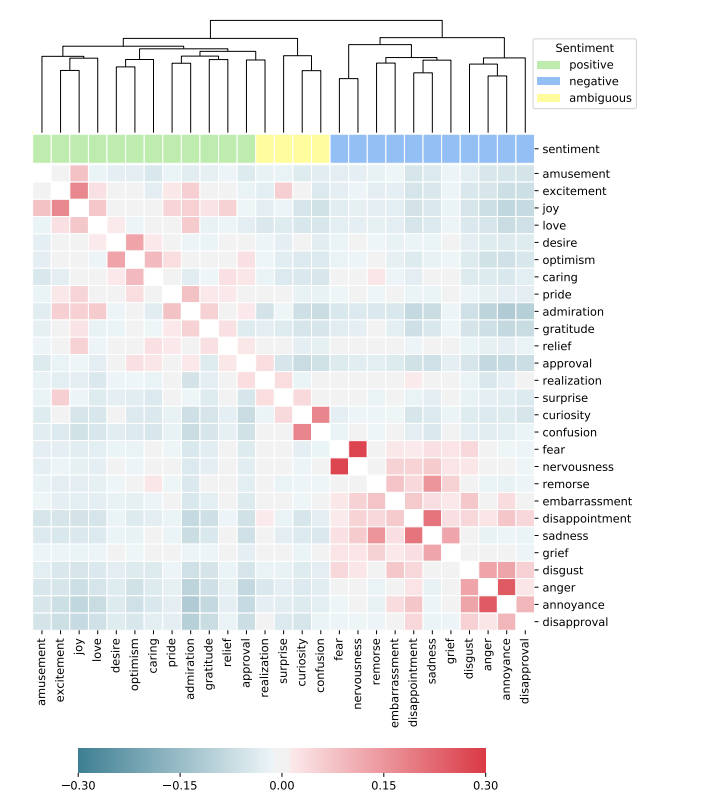
\includegraphics[width=0.7\textwidth]{Images/emotion-taxonomy.PNG}
    \caption[Hierarchical Clustering of GoEmotions Dataset]{Hierarchical clustering of the 27 emotion categories in the GoEmotions dataset\cite{demszky2020goemotions}.}
    \label{fig:goemotions_cluster}
\end{figure}

\subsection{Core Algorithmic Paradigms:} 
The implementation of the aforementioned NLP techniques relies on several core algorithmic paradigms that have become standard in modern AI research.

\subsubsection{In-Context Learning and Prompt Engineering:} 
The paradigm shift introduced by large language models like GPT-3 is their ability for \textbf{in-context learning} \cite{brown2020gpt3}. This allows models to perform new tasks based solely on information provided in their input prompt, without updating their internal parameters. This includes:
\begin{itemize}
    \item \textbf{Zero-Shot Learning:} The model is given only a natural language instruction.
    \item \textbf{Few-Shot Learning:} The model is given the instruction plus a small number of examples (N-shots) demonstrating the task.
\end{itemize}
The design of effective prompts has become a critical discipline, as the quality and structure of the input context directly determine the model's performance on downstream EI tasks \cite{amin2023affective, sabour2024emobench}.

\subsubsection{Stopping Criteria for N-Shot Learning:} 
While early stopping is used for model training, a different type of criterion is necessary for evaluating few-shot or N-shot learning performance. As the number of in-context examples ($N$) increases, performance typically improves up to a certain point before plateauing, after which adding more examples yields diminishing returns while increasing computational cost and context length \cite{brown2020gpt3}.

To systematically determine the optimal number of examples without exhaustively testing a large range, researchers have adopted specific stopping rules. A notable example is the rule applied by \cite{zhu2020stopping} , which identifies the optimal number of shots, $N^{\star}$, as the point where performance gains become negligible for two consecutive steps . This is formally defined as:
\begin{equation}
N^{\star} = \min \{ N \mid \text{F1}(N) - \text{F1}(N-1) < 0.01 \text{ and } \text{F1}(N+1) - \text{F1}(N) < 0.01 \}
\label{eq:stopping_rule}
\end{equation}
\addequation{Stopping rule for N-shot learning}

where $\text{F1}(N)$ is the F1-score achieved with $N$ in-context examples. This rule effectively identifies the "knee" of the performance curve, ensuring that the model is evaluated at a point of saturation. Adopting such a criterion, as is done in this Capstone project, provides a principled and reproducible method for comparing model performance across different granularities while balancing accuracy with efficiency.

\subsection{Fine-Tuning and Parameter-Efficient Adaptation:} 
For tasks requiring deep, specialized knowledge not fully captured during pre-training, \textbf{fine-tuning} remains a vital technique. This involves updating a pre-trained model's weights on a smaller, task-specific dataset. However, as research into scaling laws has shown, the computational cost of training and fine-tuning grows predictably with model size \cite{kaplan2020scaling}. To address the expense of updating multi-billion parameter models, \textbf{Parameter-Efficient Fine-Tuning (PEFT)} methods have been developed. A prominent PEFT technique is Low-Rank Adaptation (LoRA), which freezes the original model weights and injects small, trainable low-rank matrices into the Transformer layers. This dramatically reduces the number of trainable parameters, making it feasible to adapt large models for specialized tasks like EI on consumer-grade hardware \cite{zhao2024moei}.

\subsection{Key Algorithms for Semantic and Lexical Analysis:} 
At the heart of an LLM's ability to process language are algorithms that measure the similarity and relevance between pieces of text. These can be broadly categorized into semantic (meaning-based) and lexical (keyword-based) approaches.

\subsubsection{Semantic Similarity: Embeddings and Cosine Similarity:} 
Modern NLP systems represent text as high-dimensional vectors known as \textbf{embeddings}. These vectors are designed such that texts with similar meanings are located close to each other in the vector space. The standard method for measuring this proximity is \textbf{Cosine Similarity}:
\begin{equation}
\text{Cosine Similarity}(A, B) = \frac{A \cdot B}{\|A\| \|B\|} = \frac{\sum_{i=1}^{n} A_i B_i}{\sqrt{\sum_{i=1}^{n} A_i^2} \sqrt{\sum_{i=1}^{n} B_i^2}}
\end{equation}
\addequation{Cosine similarity}
where $A$ and $B$ are the embedding vectors. A value of 1 indicates maximum similarity, and 0 indicates orthogonality. This metric is fundamental for tasks like semantic search, text clustering, and scoring the relevance of an empathetic response \cite{xie2024empathy}.

\subsubsection{Lexical Similarity: TF-IDF and BM25:} 
While embeddings capture semantic meaning, they can sometimes miss the importance of specific keywords. Lexical algorithms address this by focusing on term frequencies. A leading algorithm in this category is \textbf{Okapi BM25} (Best Matching 25), a ranking function widely used in search engines. It scores the relevance of a document $D$ to a query $Q$ containing terms $q_1, ..., q_n$:
\begin{equation}
\text{score}(D, Q) = \sum_{i=1}^{n} \text{IDF}(q_i) \cdot \frac{f(q_i, D) \cdot (k_1 + 1)}{f(q_i, D) + k_1 \cdot \left(1 - b + b \cdot \frac{|D|}{\text{avgdl}}\right)}
\end{equation}
\addequation{BM25 scoring function}
where $f(q_i, D)$ is the term frequency of $q_i$ in $D$, $|D|$ is the document length, and avgdl is the average document length. The hyperparameters $k_1$ and $b$ control term frequency saturation and document length normalization. The Inverse Document Frequency (IDF) term is calculated as:
\begin{equation}
\text{IDF}(q_i) = \log\left(\frac{N - n(q_i) + 0.5}{n(q_i) + 0.5} + 1\right)
\end{equation}
\addequation{Inverse Document Frequency}
where $N$ is the total number of documents and $n(q_i)$ is the number of documents containing $q_i$. The literature on EI in LLMs has predominantly focused on semantic methods, leaving the potential of hybrid systems that combine the strengths of BM25 and cosine similarity largely unexplored.

\subsection{Hybrid Retrieval Approaches:} 
Recent work such as HyST demonstrates the value of combining sparse and dense retrieval signals within a single hybrid pipeline. In their framework, BM25 and dense passage retrieval (DPR) scores are fused via a weighted sum, with a parameter $\lambda$ controlling the contribution of each component. The authors report that setting $\lambda=0.5$ achieves strong performance by balancing lexical precision and semantic generalization \cite{hyst2025}. This approach highlights how sparse lexical cues and dense embeddings can complement each other.

\subsection{Evaluation Frameworks and Metrics:} 
Evaluating the performance of emotionally intelligent systems requires a robust set of metrics that capture both objective accuracy and subjective quality.

\subsubsubsection{Classification Metrics:}
For discrete tasks like emotion classification, standard metrics are used:
\begin{itemize}
    \item \textbf{True Positive (TP)}: The number of instances where the model correctly predicts the positive class (e.g., correctly identifying an emotion as "joy" when it truly is "joy").
    
    \item \textbf{True Negative (TN)}: The number of instances where the model correctly predicts the negative class (e.g., correctly identifying that a text is not "anger" when it truly is not "anger").
    
    \item \textbf{False Positive (FP)}: The number of instances where the model incorrectly predicts the positive class (e.g., predicting "sadness" when the true emotion is something else). Also known as a Type I error.
    
    \item \textbf{False Negative (FN)}: The number of instances where the model incorrectly predicts the negative class (e.g., failing to identify "fear" when it is actually present). Also known as a Type II error.
\end{itemize}

These four components form the basis of all classification evaluation metrics. Using these values, the following metrics are calculated:

\begin{itemize}
    \item \textbf{Accuracy} measures the proportion of all correctly classified instances out of the total number of instances:
    \begin{equation}
    \text{Accuracy} = \frac{\text{TP} + \text{TN}}{\text{TP} + \text{TN} + \text{FP} + \text{FN}}
    \end{equation}
    \addequation{Accuracy}
    While accuracy provides an overall performance measure, it can be misleading for imbalanced datasets where one class significantly outnumbers others.
    
    \item \textbf{Precision} measures the proportion of correct positive identifications among all instances predicted as positive:
    \begin{equation}
    \text{Precision} = \frac{\text{TP}}{\text{TP} + \text{FP}}
    \end{equation}
    \addequation{Precision}
    High precision indicates that when the model predicts a positive class, it is usually correct. This metric is important when the cost of false positives is high.
    
    \item \textbf{Recall} (also called Sensitivity or True Positive Rate) measures the proportion of actual positive instances that were correctly identified by the model:
    \begin{equation}
    \text{Recall} = \frac{\text{TP}}{\text{TP} + \text{FN}}
    \end{equation}
    \addequation{Recall}
    High recall indicates that the model successfully captures most of the positive instances. This metric is crucial when the cost of false negatives is high.
    
    \item \textbf{F1-Score} is the harmonic mean of precision and recall, providing a single, balanced measure that accounts for both false positives and false negatives:
    \begin{equation}
    \text{F1-Score} = 2 \cdot \frac{\text{Precision} \cdot \text{Recall}}{\text{Precision} + \text{Recall}}
    \end{equation}
    \addequation{F1-Score}
    The F1-Score is particularly valuable for imbalanced emotion datasets, as it penalizes extreme values in either precision or recall, ensuring that both metrics are reasonably high for a good score.
\end{itemize}
In multi-class scenarios, these are often reported as \textbf{Macro-F1} (unweighted average across classes) or \textbf{Micro-F1} (globally aggregated counts), which are sensitive to class imbalance in different ways.
\begin{equation}
\text{Macro-F1} = \frac{1}{C} \sum_{i=1}^{C} \text{F1}_i
\end{equation}
\addequation{Macro-F1}
where $C$ is the total number of classes and $\text{F1}_i$ is the F1-score of class $i$.
\textbf{Micro-F1} aggregates the contributions of all classes to compute global precision and recall before deriving the F1-score:
\begin{equation}
\text{Micro-F1} = \frac{2 \cdot \sum_{i=1}^{C} TP_i}{2 \cdot \sum_{i=1}^{C} TP_i + \sum_{i=1}^{C} FP_i + \sum_{i=1}^{C} FN_i}
\end{equation}
\addequation{Micro-F1}
where $TP_i$, $FP_i$, and $FN_i$ are the true positives, false positives, and false negatives for class $i$.
\subsection{Human-Centered and Psychometric Evaluation:} 
For subjective qualities like empathy, automatic metrics are often inadequate. The gold standard is \textbf{human evaluation}, where human raters score system outputs on scales (e.g., 1-5 Likert scale) for attributes like empathy, relevance, and helpfulness \cite{rashkin2019empathetic}.

Furthermore, recent work has introduced \textbf{psychometric benchmarks} that evaluate LLMs using tests designed for humans. This approach measures not just task performance but also the alignment of an LLM's reasoning patterns with human norms, often using the \textbf{Pearson correlation coefficient ($r$)} to quantify this alignment \cite{zhou2023emotional}.

\section{Existing Related Studies}
This section introduces the methods on how we conducted the literature review and presents a comparative analysis of key studies in the field of emotional intelligence in large language models.
\subsection{Research Methodology:} 
To provide a comprehensive analysis of the current research landscape, a Systematic Literature Review (SLR) methodology was adopted. This structured approach ensures a thorough and unbiased synthesis of existing scientific contributions. The review focused on identifying core methodologies, datasets, and key findings related to emotional intelligence in large language models. The process followed the systematic filtering stages illustrated in Figure \ref{fig:slr_steps}.

The search targeted peer-reviewed articles published between 2019 and 2025 to capture the most recent advancements in Transformer-based architectures. The primary databases consulted included:
\begin{itemize}
    \item ACL Anthology
    \item arXiv (for preprints with significant impact)
    \item IEEE Xplore Digital Library
    \item ACM Digital Library
    \item Google Scholar
\end{itemize}
Relevant studies were identified using combinations of the following keywords: "emotional intelligence LLM," "empathetic dialogue systems," "emotion recognition NLP," "affective computing transformers," "emotion cause extraction," and "sentiment analysis LLM."

%% ENHANCEMENT: Refined the TikZ diagram for a more professional and aesthetically pleasing look.
\tikzset{
  startend/.style = {ellipse, draw, line width=0.8pt, fill=blue!20, text width=3cm, align=center, minimum height=2.5em},
  process/.style  = {rectangle, draw, rounded corners, line width=0.8pt, fill=green!15, text width=2.8cm, align=center, minimum height=2.5em},
  arrow/.style    = {-Stealth, thick, rounded corners=5pt}
}
\begin{figure}[htbp]
    \centering
    \begin{tikzpicture}[scale=0.9, node distance=2.5cm and 1.5cm, transform shape]
        \node (source) [startend] {Source Identification};
        \node (search) [process, right=of source] {Keyword Search};
        \node (dedup) [process, right=of search] {Deduplication};
        \node (screen) [process, below=1.5cm of dedup] {Screening (Title/Abstract)};
        \node (review) [process, left=of screen] {Full-Text Review};
        \node (final) [startend, left=of review] {Final Selection (15 Studies)};

        \draw [arrow] (source) -- (search);
        \draw [arrow] (search) -- (dedup);
        \draw [arrow] (dedup) -- (screen);
        \draw [arrow] (screen) -- (review);
        \draw [arrow] (review) -- (final);
    \end{tikzpicture}
    \caption{Systematic Literature Review Methodology Steps}
    \label{fig:slr_steps}
\end{figure}

\subsection{Inclusion and Exclusion Criteria:} 
Papers were selected for final analysis based on the following systematic criteria:
\begin{itemize}
    \item \textbf{Timeframe:} Published between 2019 and 2025.
    \item \textbf{Technical Focus:} Primary research addressing EI capabilities in LLMs or related Transformer architectures, including classification, generation, or reasoning tasks.
    \item \textbf{Methodology:} Empirical studies with quantitative evaluation metrics, system implementations, or comparative analyses.
    \item \textbf{Exclusion:} Papers focused purely on theory, surveys without novel analysis, or studies using non-neural methods were excluded.
\end{itemize}

\subsection{Comparative Analysis by Research Axis:} 
The systematic review identified 15 key studies that collectively demonstrate the state of the art. These studies were organized into four thematic research axes to facilitate a clear comparative analysis, as summarized in Table \ref{tab:comparative_summary}.
\begin{sidewaystable}[htbp]
\centering
\scriptsize
\setlength{\tabcolsep}{2pt}
\renewcommand{\arraystretch}{0.95}
\begin{tabularx}{\textwidth}{
    |>{\centering\arraybackslash}p{0.9cm}
    |>{\raggedright\arraybackslash}p{2cm}
    |>{\centering\arraybackslash}p{0.7cm}
    |>{\raggedright\arraybackslash}p{1.8cm}
    |>{\raggedright\arraybackslash}p{1.6cm}
    |>{\centering\arraybackslash}p{0.7cm}
    |>{\centering\arraybackslash}p{0.9cm}
    |>{\raggedright\arraybackslash}X
    |>{\centering\arraybackslash}p{1.3cm}
    |>{\raggedright\arraybackslash}X|} 
\hline
\multicolumn{3}{|c|}{\textbf{STUDY}} & \multicolumn{3}{c|}{\textbf{METHODOLOGY}} & \multicolumn{2}{c|}{\textbf{DATASETS}} & \multicolumn{2}{c|}{\textbf{PERFORMANCE}} \\
\hline
\textbf{Year} & \textbf{Author} & \textbf{Ref} & \textbf{Algorithm} & \textbf{Technique} & \textbf{Shots} & \textbf{Type} & \textbf{Dataset Description} & \textbf{Emotion Cluster} & \textbf{Metrics \& Results} \\
\hline

\textbf{2019} & Rashkin et al.  & \cite{rashkin2019empathetic} & \textbf{MoEL} & Transformer empathetic dialogue & N/A & Public & \textbf{Empathetic
Dialogues} \cite{rashkin2019empathetic}: 25k conversations, speaker-listener pairs & 32 emotions & Human: 68\% empathetic \\
\hline

\textbf{2020} & Demszky et al.  & \cite{demszky2020goemotions} & \textbf{BERT} & Fine-tuning multi-label classification & N/A & Public & \textbf{GoEmotions} \cite{demszky2020goemotions}: 58k Reddit comments, fine-grained emotion taxonomy & 27 emotions + neutral & Macro-F1: 0.46 \\
\hline

\textbf{2020} & Brown et al. &  \cite{brown2020gpt3} & \textbf{GPT-3} & In-context learning & 0–32 & Public & \textbf{Multiple NLP}: SuperGLUE, WiC, etc. & Mixed (2–5 labels) & Accuracy: +30pts \\
\hline

\textbf{2021} & Liu et al.  & \cite{liu2021esconv} & \textbf{Transformer} & Emotional support dialogue generation & N/A & Public & \textbf{ESConv} \cite{liu2021esconv}: 1.3k conversations, help-seeker emotional support & 8 support strategies & Help score: +0.5 (1–5 scale) \\
\hline

\textbf{2022} & Shi et al.  & \cite{shi2022does} & \textbf{Cosine similarity} & Example selection for few-shot learning & N/A & Public & \textbf{Empathetic
Dialogues} \cite{rashkin2019empathetic}: 25k conversations for empathy modeling & Human preference & Improvement vs random selection \\
\hline

\textbf{2023} & Zhou et al.  & \cite{zhou2023emotional} & \textbf{GPT-4} & Zero-shot emotional reasoning & 0 & Public & \textbf{SECEU Test} \cite{zhou2023emotional}: Psychometric emotional intelligence assessment & N/A (test items) & EQ score: 117, correlation r=0.28 \\
\hline

\textbf{2023} & Zhan et al.  & \cite{zhan2023appraisal} & \textbf{Prompting} & Appraisal theory prediction & N/A & Private & \textbf{Private Corpus}: Emotion-appraisal pair annotations & Appraisal dimensions & Qualitative evaluation \\
\hline

\textbf{2023} & Wang et al.  & \cite{wang2023multilabel} & \textbf{BERT + cosine} & Calibration to reduce hallucination & N/A & Public & \textbf{Multi-label Sets}: GoEmotions + others & 27–32 emotions & Macro-F1: +3-5pts improvement \\
\hline

\textbf{2023} & Amin et al.  & \cite{amin2023affective} & \textbf{GPT-3.5/4} & Zero-shot evaluation on 13 tasks & 0 & Public & \textbf{Mixed datasets}: ISEAR, EmpatheticDialogues, etc. & 2–10 emotions per task & >85\% explicit, <55\% implicit emotions \\
\hline

\textbf{2024} & Wu et al.  & \cite{wu2024decc} & \textbf{DECC} & Emotion cause extraction & 3–5 & Public & \textbf{ECPE} \cite{wu2024decc}: Emotion-cause pair extraction corpus & Emotion-cause pairs & Macro-F1: +15pts improvement \\
\hline

\textbf{2024} & Xie et al.  & \cite{xie2024empathy} & \textbf{LLM} & Empathy scoring system & N/A & Public & \textbf{Empathetic
Dialogues} \cite{rashkin2019empathetic}: 25k conversations for empathy assessment & Empathy scores & Pearson correlation r≈0.7 \\
\hline

\textbf{2024} & Zhao et al.  & \cite{zhao2024moei} & \textbf{Transformer} & Modular parameter-efficient fine-tuning & N/A & Public & \textbf{EiBench} \cite{zhao2024moei}: 88 datasets, comprehensive EI benchmark & 27+ emotion categories & F1 score: +5-10pts improvement \\
\hline

\textbf{2024} & Sabour et al.  & \cite{sabour2024emobench} & \textbf{EmoBench} & Emotional reasoning benchmark & 0 & Public & \textbf{EmoBench} \cite{sabour2024emobench}: Why/How emotion reasoning tasks & Reasoning questions & GPT-4 performance < human baseline \\
\hline

\textbf{2025} & Imran et al.  & \cite{imran2025cause} & \textbf{BERT} & Domain-specific emotion cause extraction & 0 & Private & \textbf{SE ECE}: Software engineering emotion-cause corpus & Emotion-cause spans & BERTScore = 0.667 \\
\hline

\textbf{2025} & Liu et al.  & \cite{liu2025retrieval} & \textbf{Hybrid retrieval} & BM25 + dense vector example selection & N/A & Public & \textbf{Empathetic
Dialogues} \cite{rashkin2019empathetic}: 25k conversations for retrieval & Human preference evaluation & Improvement vs random baseline \\
\hline

\end{tabularx}
\caption{Comparative Summary of 15 Key EI Studies (2019–2025)}
\label{tab:comparative_summary}
\end{sidewaystable}  



\subsection{Analysis of the Current Research Landscape:}
The reviewed literature reveals significant progress in the individual components of computational EI, yet several critical gaps remain that limit the development of robust, practical, and truly intelligent systems.

\subsection{The Human-Model Reasoning Gap:}
Perhaps the most fundamental challenge identified is that even top-performing LLMs do not reason about emotions in the same way humans do. Studies utilizing psychometric benchmarks consistently find a low correlation between model response patterns and human norms, even when the model selects the "correct" answer \cite{zhou2023emotional, sabour2024emobench}. This suggests that current models are sophisticated pattern matchers that have learned the statistical correlations in language associated with emotion but lack a deeper, causal understanding of affective states. They can identify \textit{what} emotion is being expressed but struggle with the \textit{why} and \textit{how} that constitute genuine intelligence.

\subsection{The Implicit versus Explicit Signal Divide:}
A direct consequence of this reasoning gap is the stark performance difference between tasks involving explicit versus implicit emotional cues. LLMs demonstrate high accuracy when an emotion is clearly stated or triggered by unambiguous keywords \cite{amin2023affective}. However, their performance degrades significantly when they must infer emotions from subtext, sarcasm, or complex contextual situations. This limitation is a major barrier to real-world application, as human communication is rich with implicit meaning.

\subsection{Limitations of Single-Method Similarity:}
The literature demonstrates a heavy reliance on a single modality of similarity dense vector-based semantic similarity for tasks like retrieval and relevance ranking \cite{xie2024empathy, shi2022does}. While powerful, this approach has inherent limitations. Semantic embeddings can sometimes group conceptually related but factually incorrect items, and they may fail to capture the importance of specific, rare keywords that are critical for understanding context. The near-total absence of research into hybrid similarity frameworks that combine the semantic understanding of embeddings with the lexical precision of algorithms like BM25 represents a significant, unaddressed gap in the field.

\subsection{Computational Deployment and Specialization Constraints:}
While some studies showcase impressive capabilities from fine-tuned models \cite{zhao2024moei}, they often rely on extensive computational resources for training. The practical deployment of such specialized models in real-time, resource-constrained environments remains a challenge. There is a need for solutions that are not only accurate but also computationally efficient, a consideration often overlooked in pure research settings.

\subsection{Emerging Solution Requirements and Research Gaps:}
The convergence of these findings points toward specific solution requirements that emerge naturally from the limitations in existing approaches. The challenges of implicit signal processing and the limitations of single-method similarity, in particular, suggest the need for more robust information retrieval and reasoning systems.

The identified research gaps lead logically toward the exploration of a hybrid architecture. The most significant unexplored opportunity lies in the synergistic combination of semantic and lexical search. The development of a hybrid retrieval engine that integrates dense vector search (via cosine similarity) with sparse keyword search (via BM25) could offer a more robust solution. Such a system could leverage semantic embeddings to understand the general intent and emotional context of a query, while using BM25 to pinpoint specific, critical keywords, potentially overcoming the respective weaknesses of each approach. This integrated hybrid methodology forms the central motivation and core technical contribution of the present Capstone project.
\begin{table}[H]
\centering
\caption{Summary of Identified Research Gaps}
\begin{tabular}{|p{4cm}|p{4cm}|p{6cm}|}
\hline
\textbf{Dimension} & \textbf{Current Limitation} & \textbf{Gap Addressed by This Study} \\ \hline
Granularity Handling & Models evaluated on fixed emotion sets & Multi-granular evaluation (27/15/3 labels) \\ \hline
Retrieval Strategy & Single-method (semantic or lexical) & Hybrid fusion with $\lambda=0.5$ \\ \hline
Learning Evaluation & No plateau detection & Adaptive $N^{\star}$-based stopping rule \\ \hline
Interpretability & Black-box outputs & Transparent Streamlit visualization \\ \hline
Ethical Design & Minimal consideration & Built-in safeguards and explainability \\ \hline
\end{tabular}
\end{table}
\section {Conclusion}

This chapter has provided the comprehensive theoretical and empirical foundation for the present Capstone project, systematically building the case for its core research objectives. The work was organized into two primary pillars: a detailed background on the foundational concepts of computational emotional intelligence, and a systematic literature review to analyze the current state of the art.

The background section established the necessary theoretical and technical foundations for the research. It began by grounding the work in the psychological principles of emotional intelligence, primarily the Mayer-Salovey model, which provides a structured blueprint for the capabilities an emotionally aware AI should possess. Following this, the chapter detailed the core NLP techniques used in affective computing, the algorithmic paradigms such as in-context learning that dominate modern research, and the essential mathematical underpinnings of both semantic (Cosine Similarity) and lexical (BM25) analysis. Furthermore, it established the importance of structured datasets like GoEmotions and the concept of emotional granularity, which directly inform the project's experimental design.

Building upon this foundation, a systematic literature review was conducted to survey and synthesize 15 key studies from recent years. The analysis revealed a field that has made significant strides in leveraging large language models for explicit emotion recognition tasks. However, it also illuminated critical and persistent limitations. The most salient findings were the qualitative gap between model performance and genuine human-like emotional reasoning, the consistent struggle of LLMs to interpret implicit or nuanced emotional cues, and a critical under-exploration of hybrid information retrieval methodologies. The review clearly demonstrated that the field's heavy reliance on single-modality semantic similarity represents a significant, unaddressed research gap.

In conclusion, this chapter serves as the critical justification for the present Capstone project. By thoroughly reviewing the established knowledge and identifying a precise, actionable gap in the existing literature, it provides a compelling rationale for the proposed methodology. The exploration of a hybrid retrieval system that synergistically combines semantic and lexical search is not merely an incremental improvement but a direct response to a fundamental limitation in the current state of the art. The following chapter will detail the specific methodology designed to build this system and rigorously test the hypothesis that this hybrid approach can lead to a more robust and accurate model of computational emotional intelligence.

